\documentclass[letterpaper,10pt]{article}

\usepackage{titling}
\usepackage{listings}
\usepackage{url}
\usepackage{setspace}
\usepackage{subfig}
\usepackage{sectsty}
\usepackage{pdfpages}
\usepackage{colortbl}
\usepackage{multirow}
\usepackage{multicol}
\usepackage{relsize}
\usepackage{amsmath}
\usepackage{wasysym}
\usepackage{fancyvrb}
\usepackage{amssymb}
\usepackage{ifsym}
\usepackage{amsmath,amssymb,amsthm,graphicx,xspace}
\usepackage[titlenotnumbered,noend,noline]{algorithm2e}
\usepackage[compact]{titlesec}
\usepackage{XCharter}
\usepackage[T1]{fontenc}
\usepackage{tikz}
\usetikzlibrary{arrows,automata,shapes,trees,matrix,chains,scopes,positioning,calc}
\tikzstyle{block} = [rectangle, draw, fill=blue!20, 
    text width=2.5em, text centered, rounded corners, minimum height=2em]
\tikzstyle{bw} = [rectangle, draw, fill=blue!20, 
    text width=4em, text centered, rounded corners, minimum height=2em]

\definecolor{namerow}{cmyk}{.40,.40,.40,.40}
\definecolor{namecol}{cmyk}{.40,.40,.40,.40}

\let\LaTeXtitle\title
\renewcommand{\title}[1]{\LaTeXtitle{\textsf{#1}}}


\newcommand{\handout}[5]{
  \noindent
  \begin{center}
  \framebox{
    \vbox{
      \hbox to 5.78in { {\bf ECE356: Database Systems } \hfill #2 }
      \vspace{4mm}
      \hbox to 5.78in { {\Large \hfill #4  \hfill} }
      \vspace{2mm}
      \hbox to 5.78in { {\em #3 \hfill} }
    }
  }
  \end{center}
  \vspace*{4mm}
}

\newcommand{\lecture}[3]{\handout{#1}{#2}{#3}{Lecture #1}}
\newcommand{\tuple}[1]{\ensuremath{\left\langle #1 \right\rangle}\xspace}

\addtolength{\oddsidemargin}{-1.000in}
\addtolength{\evensidemargin}{-0.500in}
\addtolength{\textwidth}{2.0in}
\addtolength{\topmargin}{-1.000in}
\addtolength{\textheight}{1.75in}
\addtolength{\parskip}{\baselineskip}
\setlength{\parindent}{0in}
\renewcommand{\baselinestretch}{1.5}
\newcommand{\term}{Winter 2018}

\singlespace


\begin{document}

\lecture{ 21 --- Transaction Isolation }{\term}{Jeff Zarnett}

\section*{Transaction Isolation}

Recall from last time the idea of transaction isolation is that multiple concurrent transactions should not be able to lead somehow to an inconsistent state due to concurrent operations. The simple approach is to force transactions to run one at a time, which of course ensures that concurrency is not a problem, but also ensures that nobody uses your database because it's very slow. Previous courses have examined in some detail why you want concurrency: better performance, better resource utilization, fewer user tears. Let us waste no time discussing the particular merits of concurrency. 

The database server has the same threading problems that you likely recall from the discussion of concurrency: the operating system schedules the threads and it chooses when it is a good time for a switch between them, meaning the database does not have control over when such a switch will happen. So if two operations are in flight at a particular time, they could be executing in two different threads and switches between them can occur at arbitrary times. If anything, they will occur at the worst possible times and really cause problems.

Let's imagine that we have two transactions that are going to execute, in an example from~\cite{dsc} I've modified a bit to be a little less strange. In the original there is a transfer in the amount of 10\% of the balance from one account to another but this does not seem sensible since one normally specifies an amount to be transferred, not a percentage. In the modified example, one transaction is a transfer of \$50 from A to B, and another transaction is the calculation of monthly earned interest, wherein the lucky account holder of A receives a humongous 1\% interest on the balance in this account.

\begin{multicols}{2}
\textbf{Transaction $T_{1}$}
\begin{verbatim}
T1.1. read A.balance
T1.2. A.balance = A.balance - 50
T1.3. write A.balance
T1.4. read B.balance
T1.5. B.balance = B.balance + 50
T1.6. write B.balance
\end{verbatim}
\columnbreak
\textbf{Transaction $T_{2}$}

\begin{verbatim}
T2.1 read A.balance
T2.2 A.balance = A.balance * 1.01
T2.3 write A.balance
\end{verbatim}

\end{multicols}

This sort of multi-column pseudo code concurrency problem may be reminding you of unpleasant memories of learning about concurrency. Well, we still have the usual problem here. An improper interleaving of two statements means one of the changes gets lost, and the \$50 is not deducted or the interest is not calculated at all. 

This pair of transactions is interesting in that there are two correct answers. Suppose the initial value in account A is \$2000. If the transactions are executed serially, first $T_{1}$ then $T_{2}$, then the \$50 is deducted and the interest is calculated on \$1950  and the total amount is \$1969.50. If the transactions are executed serially but in the opposite order, then the interest is calculated on \$2000 and then the \$50 is deducted, meaning the total balance at the end is \$1970.00, a difference of 50 cents. Both answers are correct in the sense that they are consistent.

These two execution sequences are called \textit{schedules} and they represent a chronological ordering in which instructions are executed~\cite{dsc}. A schedule is called valid if it does not break any of the rules and cannot cause some inconsistent state. A serial schedule means one transaction runs to completion before the next begins and for $n$ transactions there are $n!$ different valid serial schedules. Probably you have noticed however, that the operations on the A account are finished in $T_{1}$ after statement \texttt{T1.3} and you could in theory start the second transaction a little bit early to get some performance increase. Well -- maybe! That might be revealing the partial state of a transaction and that might not be acceptable; what if an error is encountered on assigning the balance of B because and the transaction is to be rolled back? Things start to get interesting...

We do not actually need for all transactions to be done serially, but they do need to be \textit{serializable}, which means there must exist an equivalent serial schedule~\cite{dsc}. That means the end result when all is said and done must be the same as if the transactions executed in a serial order (any serial order). So the following order is acceptable because it is equivalent to the serial schedule of first $T_{1}$ and then $T_{2}$:

\begin{verbatim}
T1.1. read A.balance
T1.2. A.balance = A.balance - 50
T1.3. write A.balance
T2.1 read A.balance
T2.2 A.balance = A.balance * 1.01
T2.3 write A.balance
T1.4. read B.balance
T1.5. B.balance = B.balance + 50
T1.6. write B.balance
\end{verbatim}

But the following order is not okay because it does not match either $T_{1}$ then $T_{2}$ or $T_{2}$ then $T_{1}$:

\begin{verbatim}
T1.1. read A.balance
T1.2. A.balance = A.balance - 50
T2.1 read A.balance
T2.2 A.balance = A.balance * 1.01
T2.3 write A.balance
T1.3. write A.balance
T1.4. read B.balance
T1.5. B.balance = B.balance + 50
T1.6. write B.balance
\end{verbatim}

If this order were executed, the balance would be \$1950.00, meaning the calculation of the interest would be lost altogether, an unacceptable outcome. And looking at the value of \$1950.00 we can verify it is neither \$1969.50 nor \$1970.00 and is therefore equivalent to neither schedule. 

\subsection*{Determining Serializability}

If our intention is to ensure serializability, we do need to know how to tell if a schedule is serializable. For simple examples like above, we can determine by inspection whether it is serializable and if pressed to do so on an exam could back that up with the reasoning showing that a certain schedule produces the same results as $T_{1}$ then $T_{2}$. Those are the simple cases; when multiple transactions are interleaved it starts to get more difficult.

From the view of the database (or any program, really), it is more or less irrelevant what the contents of a variable or attribute are. The order reads and writes are what matter; the actual value is pretty much irrelevant. In the previous examples, it changes nothing if the amount transferred is \$5 or \$500, or if the interest rate is 1\% or 3\%, or if the starting balance is \$1000 or \$2000. It is the read and write operations themselves that need ordering.

In the textbook~\cite{dsc} they are called something else but to use terminology consistent with the other courses that touch on this sort of conflict, we call them ``hazards'' and there are four possibilities.

\begin{enumerate}
	\item \textbf{RAW} (Read After Write) - The classic form of dependency. The read has to take place after the write, otherwise there's nothing to read, or an incorrect value will be read.
	\item \textbf{WAR} (Write After Read) - A write cannot take place until the read has happened, to ensure the read takes the correct value.
	\item \textbf{WAW} (Write After Write) - A write cannot take place because an earlier write needs to happen first. If we do them out of order, the final value may be out of date or otherwise incorrect.
	\item \textbf{RAR} (Read After Read) - No such hazard! 
\end{enumerate}

Yup, reads don't interfere with one another in any way, and why would they; that one transaction reads the value has no impact on a future read. But writes always cause a hazard. Two transactions $T_{i}$ and $T_{j}$ are said to \textit{conflict} if they are operations by different transactions on the same data, and at least one of those operations is a write. It does have to be the same data, of course, otherwise there is no conflict.

Non-conflicting instructions can be swapped with no consequences in the schedule. If a schedule $S$ can be transformed into $S'$ by a series of swaps of non-conflicting instructions, we say that $S$ and $S'$ are conflict-equivalent~\cite{dsc}. If a particular schedule $S$ is conflict-equivalent to a serial schedule then it is called conflict-serializable~\cite{dsc}. In general we need a particular schedule to be conflict-serializable, not serial; that is enough to make sure we can perform the operations and get consistent results.

\paragraph{Determining conflict-serializability.} A simple approach to determining the conflict-serializability of a schedule relies on building a directed graph called a precedence graph. This is formed out of the transactions participating in the schedule and constraints are reflected as edges in this graph. Each transaction is a node. If transaction $T_{i}$ does a read before transaction $T_{j}$ does a write, that is an edge from $T_{i}$ to $T_{j}$. The same holds for a read after write dependency and for a write after write dependency. 

If this sounds a lot like a resource allocation graph, it's because it is. The resource allocation graph was used to detect deadlock by looking for a cycle. Here, we will still search for a cycle, because the presence of a cycle means that the schedule is not conflict-serializable. As before, known graph theory algorithms are perfectly suitable for detecting a cycle.

The following two graphs show very simple precedence graphs for two transactions~\cite{dsc}:

\begin{center}
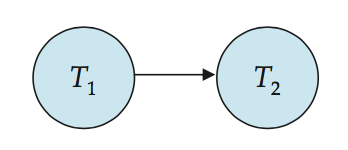
\includegraphics[width=0.25\textwidth]{images/precedence-1}
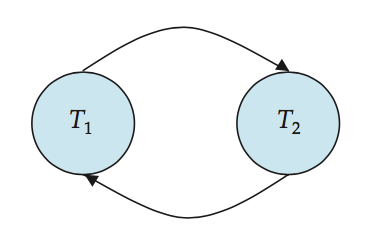
\includegraphics[width=0.25\textwidth]{images/precedence-2}
\end{center}

Once the precedence graph has been assembled, it is fairly easy for humans to figure out a valid serial ordering of the transactions. Topological sorting is the name of the graph algorithm to get a linear ordering of the transactions. Remember that the sort order of the transactions does not mean that they are actually executed in that order completely; it is just that the execution is conflict-equivalent to the linear execution order. 

If a cycle is detected, a topological sort is not possible: it cannot be turned into a linear ordering of transactions. That should be fairly obvious, but needs to be noted.

A diagram showing a precedence graph and two valid topological sorts is shown below~\cite{dsc}. Suppose we have four transactions. From that, a topological sort is performed to get the linear order of transactions.

\begin{center}
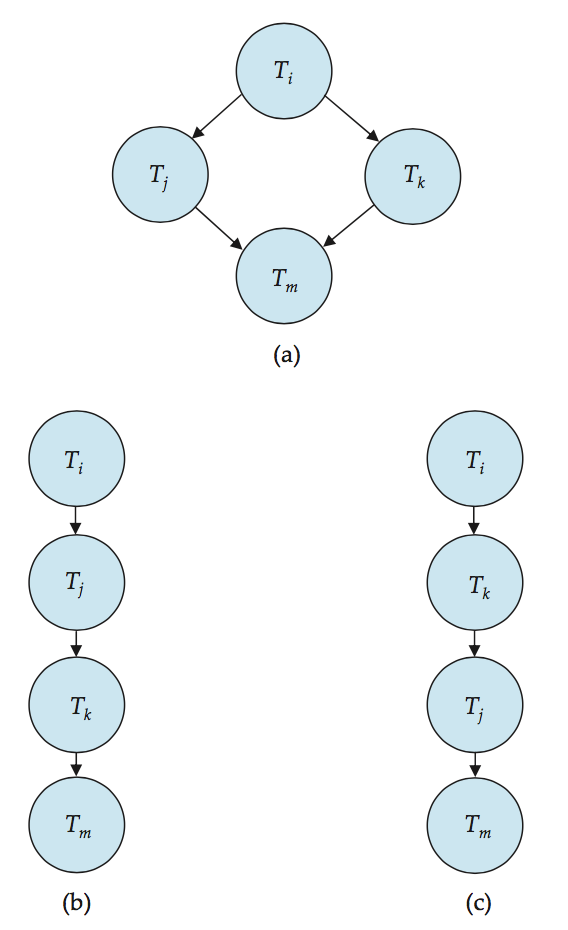
\includegraphics[width=0.35\textwidth]{images/topological}
\end{center}

Both (b) and (c) in this diagram are valid serial schedules. They are not equivalent, but that is okay, they do not have to be. Either option is fine when it comes to executing the transaction. They may or may not result in the same final state, but they will always result in consistent state.

\subsection*{Isolation and Atomicity}

If we have a schedule that is not serial but conflict-equivalent to one, we have a potential problem that we did not have before. Suppose we have two transactions that are running in parallel and we have a schedule that is conflict equivalent to first $T_{1}$ then $T_{2}$. What if transaction $T_{1}$ writes a value, then $T_{2}$ reads that value, but $T_{1}$ aborts immediately afterwards and needs to be rolled back? For example, $T_{1}$ subtracts the \$50 and $T_{2}$ calculates the 1\% interest; if the subtraction transaction is aborted, then the calculation of interest may not use the updated value in its computation. But what if it has already read it? We have a problem!

We would like to know what schedules make recovery possible at all, and even which schedules make recovery relatively simple~\cite{fds}. If we can recover from a problem, the schedule is called \textit{recoverable}. A schedule that is not recoverable should never be chosen by the database server because it means a transaction that is aborted could potentially result in inconsistent results, violating the atomicity principle.

On the other hand, if a transaction $T_{k}$ is committed, it should never be necessary to roll that transaction back~\cite{fds}. If we did, the durability property would be violated. Commit is final and we do not want that policy to be violated.

The behaviour we are looking for in the example is that if $T_{1}$ aborts for some reason, $T_{2}$ must also abort. The second transaction is dependent on the first. Thus  $T_{2}$ cannot commit until $T_{1}$ has committed. The general statement of this principle is that the schedule is recoverable as long as no transaction $T$ commits until all transactions $T'$ that precede it have committed. ``Precede'' in the previous sentence refers to our idea of the precedence graph.

The placement of the commit operations is what makes a schedule recoverable. So in addition to paying attention to the placements of the read and write operations, the placement of the commit operations matters too. All of this is distinct from the idea of actually performing the recovery; how the transactions are rolled back is independent of the fact that we need to actually perform that rollback. If sufficient information is kept in the log then it does make the rollback possible (but not very pleasant).

If we have two transactions as above like $T_{1}$ and $T_{2}$ and the first transaction aborts, it may cause the second transaction to abort. That may not sound like a problem, but if there are a lot of transactions in flight at the same time, a transaction that aborts may cause some other transactions to abort, which would in turn cause more transactions to abort. This is called a cascade rollback. This can easily cause a lot of time to be wasted since so much work needs to be done to undo the transactions that cannot be completed.

It may be desirable, where possible, to prevent the need to cascade rollbacks. A schedule will be \textit{cascadeless} (i.e. contain no cascade rollbacks) if every transaction only reads items that have already been committed. It should be easy to convince yourself that if that is the case, then a cascade rollback can never occur. If transaction $T$ reads an item written by $T'$, then either (1) $T'$ commits, in which case the transaction cannot abort and there is no problem, or (2) $T'$ aborts and the read by $T$ has not yet taken place. It does delay $T$ but ensures no cascading rollback. There is, of course, potentially reduced performance of normal transactions to avoid a very costly cascade rollback. 

There is a third, even more restrictive schedule called a \textit{strict schedule} in which transactions may neither read nor write a data element until the last transaction that writes that element has committed (or aborted)~\cite{fds}. This even more restrictive schedule means that it will be relatively easy to recover if we must. Suppose the field $x$ is initially 1 and $T_{3}$ writes 3 into $x$ and then $T_{4}$ writes 5 into $x$. If $T_{3}$ aborts the rollback might set the value of $x$ back to 1 meaning the $T_{4}$ change is lost. A strict schedule avoids this.

As a strict schedule is defined as an additional restriction on a cascadeless schedule, it is trivial to show that the strict schedule is also cascadeless.  And a cascadeless schedule is always recoverable (also trivial to show). 

\subsection*{Transaction Isolation Levels}

Serializability is how the database server ensures that data operations produce consistent results. As there are performance costs that come with performing things strictly, we will sometimes allow a little bit of rule-breaking to allow better performance... This is dangerous, and it means that more care needs to be taken on the part of the developers: if they want to use this sort of feature they need to be responsible about its use.

The isolation levels specified in the SQL standard are~\cite{dsc}:
\begin{itemize}
	\item \textbf{Serializable}: ensures serializable execution (although some databases don't necessary fulfill this...)
	\item \textbf{Repeatable read}: allows only committed data to be read and further requires that if the transaction reads a data item $x$ twice, those two reads may not have another transaction that writes $x$ between them.
	\item \textbf{Read committed}: allows only committed data to be read, but does not require repeatable reads.
	\item \textbf{Read uncommitted}: allows uncommitted data to be read.
\end{itemize}

All isolation levels above also forbid writing a data item that has already been written by another transaction that has not yet been committed (or aborted). The transaction isolation level is often set at ``read committed'' but it can be changed by some syntax in SQL if the application developer wishes to allow better performance~\cite{dsc}. We will come back to the subject of how to actually implement the isolation levels in the next topic.

Non-repeatable reads tend to happen in real life a lot. An example from~\cite{dsc} illustrates using the common example of selecting seats on a flight, but it could also apply to buying concert tickets, or online shopping. When you go to select seats, you are presented with a map and you get to make your choice about which seat. If multiple people are doing the same thing then there is no problem unless two people are trying to choose the same seat. If that's not the case, then there is no conflict. If they are choosing the same seat, there might be a slight problem: both people cannot have the same seat, no matter how much the airlines would really really like to sell the same seat twice.

Ultimately, one user will succeed and the second user will not. The successful user will be told of the success and the unsuccessful user will be prompted to say select again, and be presented with the updated map. This is a form of rollback, really: the potential changes are not committed and anything attempted is undone; the user then may choose whether to give up or try again. Chances are the user does try again (they still want to get on that flight, don't they?) but they will need to make some changes before submitting again. In a rather unpleasant scenario, the user may be forced to try several times before succeeding.

We could force serializability by allowing only one passenger to select seats at a time. That might be acceptable (if annoying) if seat selection took place only at the time when flights are booked. That isn't what happens, though; people select them at check-in. In that case we let the users make edits, but the process of actually updating the database runs in transactions, and those transactions need to be serialized. 

This problem is a general one when we have client applications interacting with data stored in the database. The stored data is called up and sent to the client for editing. If some other client is accessing that data at the same time, there is a conflict. Before changes are applied, it is common to reload the underlying data and see if it has changed; if so then the current edit cannot go through without some sort of confirmation or changes. Serializability occurs only on the parts that happen in the database; the user changes are all considered concurrent (for our definition of concurrent in previous classes: no defined order).

To actually achieve the isolation levels, there are three strategies in~\cite{dsc} that we can discuss: locking, timestamps, and snapshot isolation.

\paragraph{Locking.} Locking is pretty much what you would expect: synchronization primitives are established and then they need to be acquired and released as is appropriate. Locks may be implemented at various granularities: one lock for the whole database, one per table, or perhaps one per tuple (but that is a headache). 

Suppose we have locks for each table. If we need more than one table, we have the possibility of a deadlock. Remember from the discussion of concurrency the idea of two-phase locking. A transaction attempts to acquire all the locks it needs and is informed of success or failure for each; if it fails to acquire any of them, it will release the ones it has acquired and then try again. 

We can also have reader-writer locks which could speed up execution of the transaction as well, especially if reads are much more common than writes.


\paragraph{Timestamps.}  Timestamps are pretty simple; each transaction is assigned a timestamp, typically when it begins. Each data item has a read-timestamp and a write-timestamp, which are updated when the item is read our written respectively. The database server can then ensure that transactions that conflict are executed in order of the timestamps, and, failing that, aborting (and possibly restarting) the transaction.

\paragraph{Snapshot Isolation.} We have already, to some extent, discussed the idea of snapshot isolation. When a transaction is to begin, a copy is made of the data needed and the copy is modified, and then finally the modified version is committed (or aborted). This avoids the need for locking of tables, since each transaction gets its own copy of the data.

This does have a potential drawback: too much isolation! If there are two concurrent transactions, it may happen that neither transaction can ``see'' the updates from the other, and the final state is then inconsistent in some way (i.e., not equivalent to a serializable execution). That is something we will see in the discussion of concurrency control; our next topic.


\bibliographystyle{alphaurl}
\bibliography{356}


\end{document}
